\documentclass{article}
\usepackage[utf8]{inputenc}
\usepackage{graphicx}
\usepackage{float}
\usepackage{amsmath}
\usepackage[paper=a4paper,margin=1in]{geometry}
\usepackage[table,xcdraw]{xcolor}


\title{Image Segmentation}
\author{David Štych\\ Aleksandra Jamróz}
\date{\today{}}



\begin{document}
\maketitle

\section{Introduction}
During laboratory 3. of the Audio Processing, Video Processing, and Computer vision course, we faced the image segmentation problem. Our task was to perform cell recognition on a dataset of 40 microscopic images. We received the default code and then expanded it with various techniques to improve its accuracy. 


\section{IoU comparision}
The indicator of our performance was IoU (intersection over union). You can see the gathered results of successive techniques in the table below.  

\begin{table}[H]
\centering
\begin{tabular}{|
>{\columncolor[HTML]{FFFFFF}}l |c|c|}
\hline
\cellcolor[HTML]{C0C0C0}{\color[HTML]{000000} \textbf{Technique}} & \cellcolor[HTML]{C0C0C0}{\color[HTML]{000000}  \textbf{\begin{tabular}[c]{@{}c@{}}Performance \\ (IoU)\end{tabular}}} \\ \hline
{\color[HTML]{000000} Baseline system}                               & {\color[HTML]{000000} 0.6850}                                                                                                                                                        \\ \hline
{\color[HTML]{000000} Technique 1\ \ \ \ \ \ \ \ \ \ \ \ \ \ \ \ \ Changing a Gaussian filter to a median filter}                                   & {\color[HTML]{000000} 0.7125}                                                                                                                                                        \\ \hline
{\color[HTML]{000000} Technique 1 and 2\ \ \ \ \ \ \ \ \ Changing default algorithm to watershed}                           & {\color[HTML]{000000} 0.7651}                                                                                                                                                        \\ \hline
{\color[HTML]{000000} Technique 1, 2 and 3\ \ \ \ \ \ Adding dilation-erosion postprocessing}                           & {\color[HTML]{000000} 0.7815}                                                                                                                                                        \\ \hline
\end{tabular}
\end{table}

In the following paragraphs, we will provide more details about the techniques used.

\section{Preprocessing}

The default way to preprocess the images was a Gaussian filter. We used median filter instead and added contrast-limited adaptive histogram equalization (CLAHE).

\section{Automatic segmentation algorithm}
We used the watershed algorithm for segmentation. However, we very quickly encountered a problem. The cells were joining together and thereby lowering the IoU score. We attempted to solve this issue using a distance transform from the OpenCV library.

Firstly, we do Otsu thresholding to find all the cells. To this mask, we apply a distance transform function. We again applied a threshold to this image, which attempts to identify each cell. At this point, we have identified the background confidently, and centers of cells (almost definitely a foreground), and we feed those markers into a watershed algorithm.

Using this technique, we managed to separate cells in a substantial part of the dataset.


\section{Postprocessing}
We saw that some recognized cells were not full, meaning they contained holes. They appeared because cells had non-uniform colors. Some darker spots can be seen on their structure. We decided to try various morphological operations on generated masks. In the final version, we performed dilation and erosion because it resulted in the best IoU. We conducted some experiments with opening and closing images, but the improvement was relatively poor, or there was no improvement at all.

This technique worked significantly better also after adding labels expanding to our masks. Those two techniques combined visibly improved our performance.

\section{Conclusion}
The baseline technique had an average IoU of 0.685. We improved the baseline technique by 14\% (to 0.7815) according to the average IoU metric.

The first improvement was by using a median filter instead of a Gaussian filter. The most significant impact on the IoU had a change in the segmentation algorithm. Which tried to distinguish each individual cell unline a simple Otsu threshold method. Another improvement was achieved by postprocessing the predicted mask. 

The toughest problem for us were overlapping cells. Algorithm correctly divided them from the background, but couldn't distinguish them from each other. It often worsened our results and we still see place for improvement here.

\newpage
\section{Sample pictures}
During modifying the methods we wanted to have better view, in which direction to go. For that reason we implemented additional work-function to show worst and best pictures. The image on the left is correct provided mask, image on the right is mask predicted by us. 


\subsection{Worst pictures}
\begin{figure}[H]
\centering
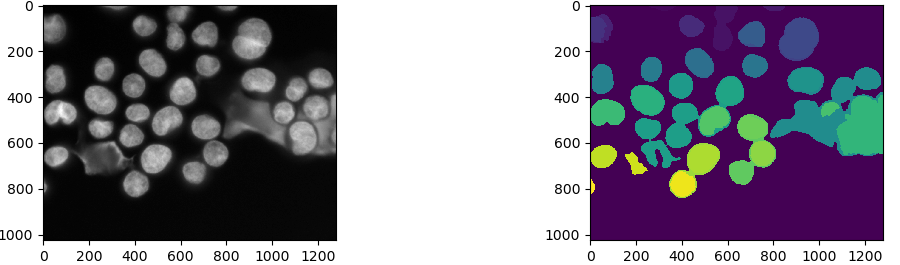
\includegraphics[width=\textwidth]{figures/1_worst.png}
\caption{The worst picture - IoU 0.588}
\end{figure}

\begin{figure}[H]
\centering
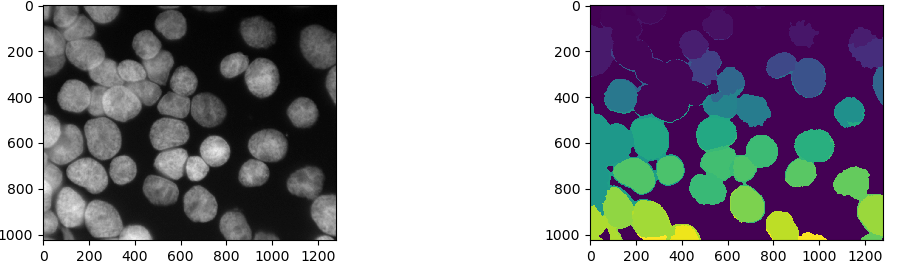
\includegraphics[width=\textwidth]{figures/2_worst.png}
\caption{Second worst picture - IoU 0.625}
\end{figure}


\begin{figure}[H]
\centering
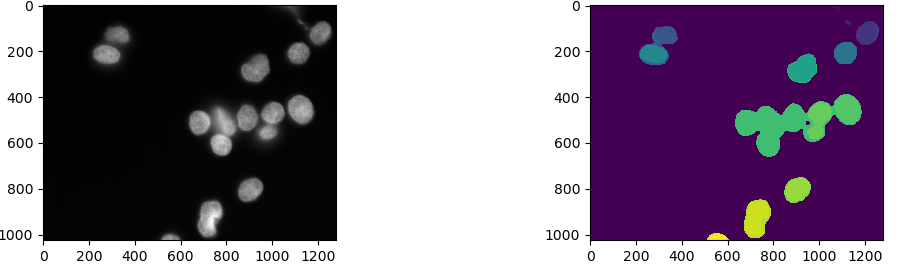
\includegraphics[width=\textwidth]{figures/3_worst.png}
\caption{Third worst picture - IoU 0.631}
\end{figure}



\subsection{Best pictures}
\begin{figure}[H]
\centering
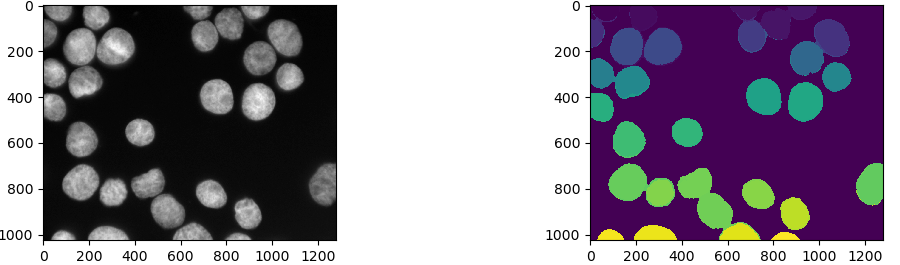
\includegraphics[width=\textwidth]{figures/1_best.png}
\caption{The best picture - IoU 0.937}
\end{figure}

\begin{figure}[H]
\centering
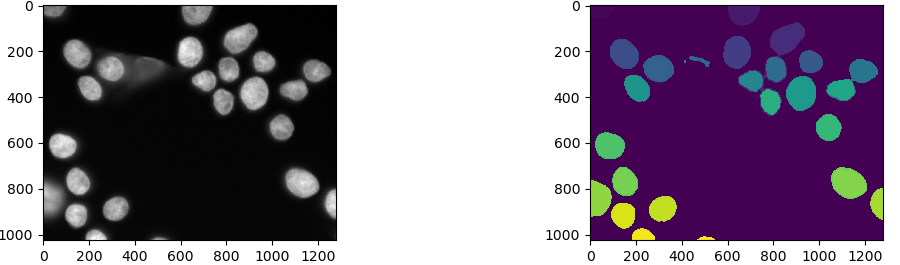
\includegraphics[width=\textwidth]{figures/2_best.png}
\caption{Second best picture - IoU 0.893}
\end{figure}


\begin{figure}[H]
\centering
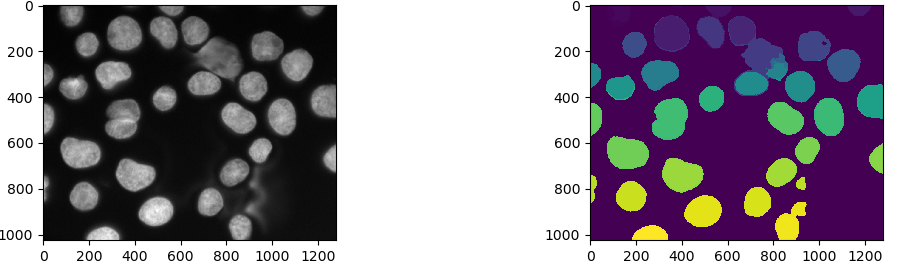
\includegraphics[width=\textwidth]{figures/3_best.png}
\caption{Third best picture - IoU 0.889}
\end{figure}


\end{document}
